\section{The Sub-Graph Method}
\label{sec:subgraph}

% \subsection{Motivation}

Both of the above improvements maintain completeness and optimality. However, there are situations, where too many possibilities for an agent's location remain, which may overwhelm the underlying solver. The motivation of~\cite{AAMAS_corridors} can be seen in Figure~\ref{fig:diagonal}. The agent is placed on a 4-connected grid going from one corner to the diagonally opposite corner. With just one agent and no obstacles, there are $\binom{2(N-1)}{N-1}$ possible shortest paths on an $N \times N$ grid. As shown in the figure, preprocessing finds out at what timesteps the agent can be located at which vertices. However, the number of choices is still too large for the solver. The idea is to pick just one of the shortest paths and to treat the other vertices as impassable obstacles. So, for these vertices, no variables enter the solver. This pruning is shown in Figure~\ref{fig:diagonal_path}.
%
\begin{figure}[ht]
\centering
\hspace{0.9cm}
\begin{subfigure}{0.27\columnwidth}
\centering
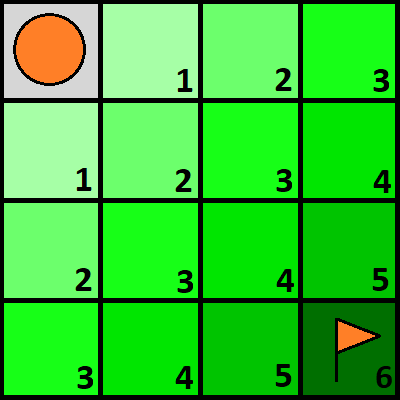
\includegraphics[width=\textwidth]{img/diagonal_agent.png}
\caption{}
\label{fig:diagonal}
\end{subfigure}
\hfill
\begin{subfigure}{0.27\columnwidth}
\centering
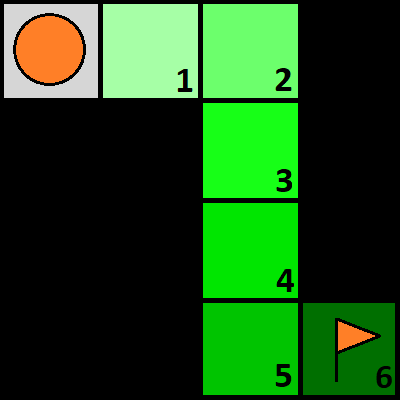
\includegraphics[width=\textwidth]{img/diagonal_single_path.png}
\caption{}
\label{fig:diagonal_path}
\end{subfigure}
\hspace{0.9cm}
\caption{An agent moving on a grid map from a corner to the opposite one. The numbers represent at what timesteps the agent can reach the given vertex.}
\label{fig:diagonal_example}
\end{figure}
%
%Another example can be seen in Figure~\ref{fig:two_agents}. The two agents have different lengths of shortest paths. For the orange agent with the longer path, the preprocessing correctly finds the only shortest path. However, the blue agent with a much shorter path may move anywhere in the shaded area. Recall that we are computing makespan optimal solutions, so we are interested in the timestep when all agents are at their goal locations. If we use the pruning technique the number of choices again reduces dramatically. The blue agent can still choose when to move to the goal location, or even move back and forth a few times, however, it may use significantly fewer vertices.
%
%\begin{figure}[ht]
%\centering
%\hspace{0.9cm}
%\begin{subfigure}{0.25\columnwidth}
%\centering
%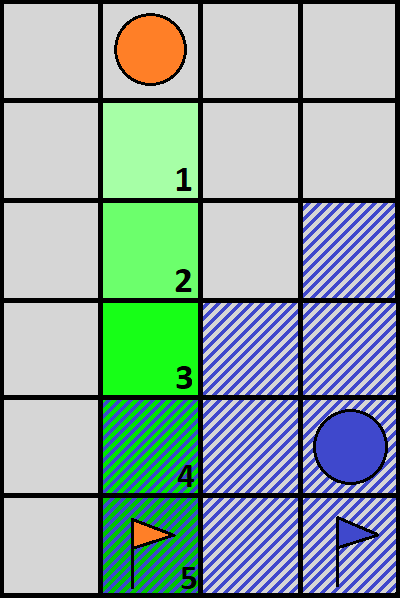
\includegraphics[width=\textwidth]{img/two-agents.png}
%\caption{}
%\label{fig:two_agents}
%\end{subfigure}
%\hfill
%\begin{subfigure}{0.25\columnwidth}
%\centering
%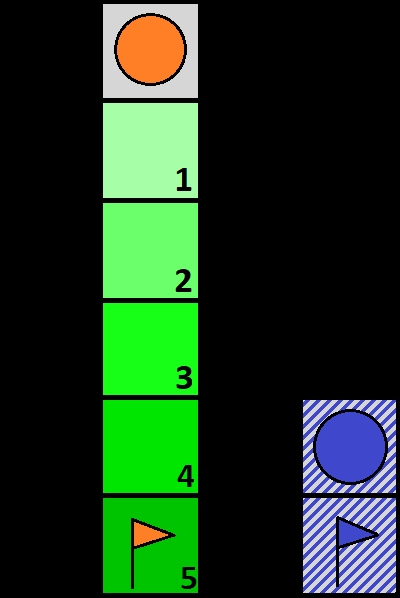
\includegraphics[width=\textwidth]{img/two-agents-path.png}
%\caption{}
%\label{fig:two_agents_path}
%\end{subfigure}
%\hspace{0.9cm}
%\caption{An instance with two agents, one with longer path allowing the other to move more freely.}
%\label{fig:two_agents_example}
%\end{figure}

Of course, this pruning does not maintain completeness in general. A simple counterexample is given in Figure~\ref{fig:m_counterexample}. The two agents want to swap their location (ie. their goal location is identical with the starting location of the other agent). To do this, the only solution is for both of them to travel to the right and use the top vertex to switch their position. %If we were to use our pruning technique, this would not be possible, making the example unsolvable.
To mitigate these instances, several strategies are proposed to change which vertices are pruned.
%
\begin{figure}[ht]
\centering
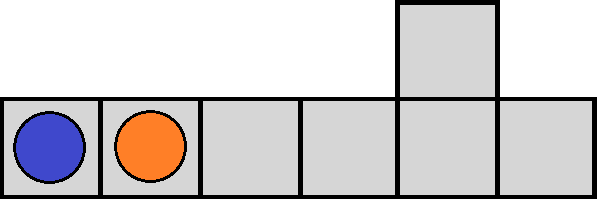
\includegraphics[width=0.45\columnwidth]{img/m_counterexample.png}
\caption{An instance with two agents that want to swap their positions.}
\label{fig:m_counterexample}
\end{figure}
%
%%% Local Variables:
%%% mode: latex
%%% TeX-master: "main"
%%% End:

\subsection*{Solving Strategies}
%
%First, we start by explaining the solving strategies used in the initial study on the graph pruning technique [citation omitted].%~\cite{TODO}.
%
% We use the following notation.
Let $SP_i$ be the set of vertices on a chosen shortest path for agent $a_i \in A$ (ie.\ a single shortest path from $s_i$ to $g_i$). The length of the path is $|SP_i|$. The union of vertices on the shortest paths of all agents is $SP_A = \bigcup_{a_i \in A} SP_i$. Note that we consider a single shortest path for each agent. If multiple shortest paths exist for an agent, one is chosen at random. Given this, the lower bound on the makespan of an instance $(G,A)$ is $LB_{mks}(G,A) = \max_{a_i \in A} |SP_i|$. For short, we refer to such lower bound just by $LB$.
%
%\begin{figure}[ht]
%\centering
%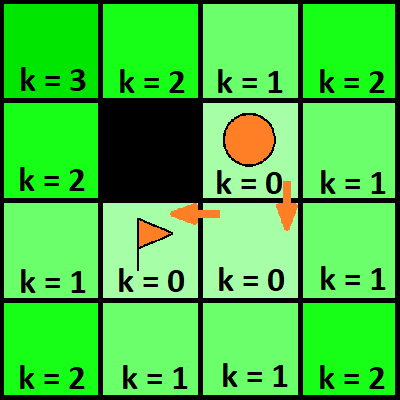
\includegraphics[width=0.37\columnwidth]{img/corridor.png}
%\caption{An instance with a single agent. Each vertex is labeled into which k-restricted graph it belongs.}
%\label{fig:corridor_width}
%\end{figure}

A \emph{k-restricted graph} $\mathit{Gres}_{k}^{SP_A}$ is a subgraph of $G$ containing only vertices $SP_A$ and vertices at most distance $k$ away from some vertex in $SP_A$. %, ie. $Gres_{k}^{SP_A} = \{v \in V \: | \: \exists u \in SP_A, \: dist(u,v) \leq k\}$.
Since we always fix $SP_A$, we write for simplicity only $\mathit{Gres}_k$. Note that $\mathit{Gres}_k \subseteq \mathit{Gres}_{k'}$ for $k \leq k'$. %An example of k-restricted graph can be seen in Figure~\ref{fig:corridor_width}. For a 0-restricted graph, only the shortest path is part of the graph. A 3-restricted graph is the whole initial graph in this case.

We define a \emph{makespan-restricted} MAPF instance as $\inst = (G,A,H)$. %This is the same problem as finding the solution for $\inst = (G,A)$ in makespan $H$.
A makespan optimal solution is found by iteratively increasing the makespan.
%
The \emph{(k,m)-relaxation} of $\inst$ is the makespan-restricted MAPF instance
\[
  \mrelax{\inst}{k}{m} = (\mathit{Gres}_k,A,LB+m)
\]
This relaxation considers only $\mathit{Gres}_k$ instead of the whole graph $G$. We find a solution with extra makespan $m$ -- extra over the lower bound on makespan. Also note that $\mathit{Gres}_k$ is constructed such that $LB_{mks}(G,A) = LB_{mks}(\mathit{Gres}_k,A)$ for any $k$, therefore, we do not need to change the notation of $LB$.

We build a partial order $\mrelaxle$ over the ($k$,$m$)-relaxations $\mrelax{\inst}{k}{m}$ such that
\[
\mrelax{\inst}{k}{m} \mrelaxle \mrelax{\inst}{k'}{m'}
\]
if $k \leq k'$, $m\leq m'$ and $k+m < k'+m'$

There is an upper bound on $k$ such that for some $k_{max}$ we have $\mathit{Gres}_{k_{max}} = G$. There is also an upper bound on the makespan for a given MAPF instance of $\mathcal{O}(V^3)$~\cite{pebble_motion}. %, however, in this paper we work only with solvable instances (this can be checked by polynomial-time algorithm) and we do not need to know the exact upper bound on makespan.
For example, assume that $k_{max}=3$ and $m_{max}=2$. Then, Figure~\ref{fig:example-relax} depicts the space of possible relaxations induced by $\mrelaxle$. Note that the partial ordering forms a lattice.
%
\begin{figure}[h]
  \centering
  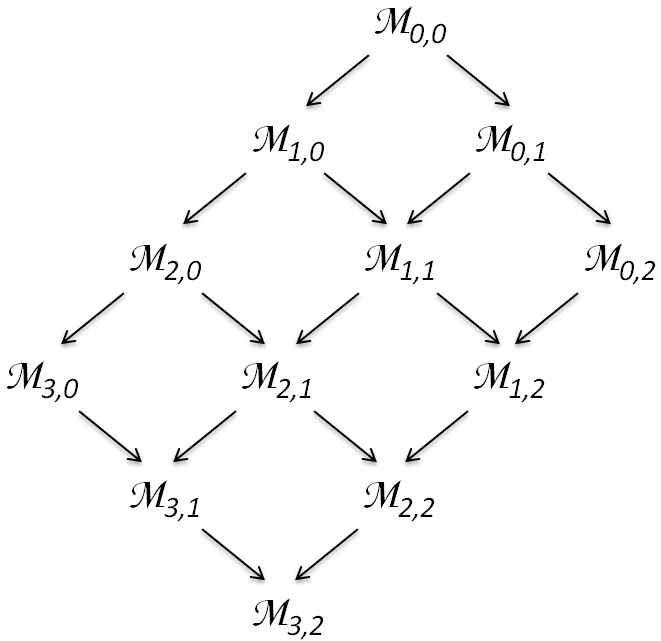
\includegraphics[width=0.65\columnwidth]{img/km_relax}
  \caption{Instance relaxations for \(k_{max}=3, m_{max}=2\).}
  \label{fig:example-relax}
\end{figure}

The generic algorithm to solve MAPF using the relaxed instances is as follows. First, we build an initial ($k$,$m$)-relaxation and we iteratively change $k$ and $m$ until the instance is solvable. This corresponds to a traversal of the lattice formed by the partial ordering $\mrelaxle$. Note that the shortest path for each agent is fixed for all of the iterations.

Next, we identify four reasonable traversals.
%
% \begin{algorithm}
%\caption{Generic algorithm solving MAPF using relaxation.}
%\label{alg:relaxation}
%\begin{algorithmic}
%\Function{Generic MAPF relaxation}{$\inst=(G,A)$}
% \State $LB = \max_{a_i \in A} |SP_i|$
% \State $(k,m) \gets Initial\_Candidate()$
% \While{not solve\_MAPF($\mrelax{\inst}{k}{m}$)}
%  \State $(k,m) \gets Relax()$
% \EndWhile
% \State \Return $LB + m$
%\EndFunction
%\end{algorithmic}
%\end{algorithm}

\textbf{Baseline Strategy.}
%
The classical approach to solving MAPF makespan optimally can be expressed in the relaxed instances as follows. We start with an initial candidate of $k_{max}$ (ie. the whole graph $G$) and $m=0$. If the relaxed instance is unsolvable, only the additional makespan $m$ is increased to $m+1$. %In terms of the Figure~\ref{fig:example-relax}, the first solved relaxation is $\mrelax{\inst}{3}{0}$ and then we are moving only to the right-hand side.
We shall refer to this strategy as \emph{baseline} or \ssb{} for short.
%
\begin{prop}\label{prop:baseline}
If a MAPF instance $\inst$ has a solution, \emph{baseline} strategy finds an optimal solution.
\end{prop}

%\begin{proof}
%Since $\inst$ has a solution, there needs to be an optimal solution with some makespan $H$ such that $LB \leq H$. The \emph{baseline} strategy will try all of the possible makespans $LB, \dots, H$, with $H$ being the first solvable.
%\end{proof}

\textbf{Makespan-add Strategy.}
%
The first smarter solution is to keep only the vertices on the shortest paths and the immediately adjacent ones. The initial candidate is $k=1$ and $m=0$. Otherwise, the strategy is the same as the baseline strategy: if the relaxed instance is unsolvable, we increase $m$ to $m+1$ while $k$ is never changed. We refer to this strategy as \emph{makespan-add} or \ssm{} for short.
%
\begin{prop}\cite{AAMAS_corridors}
The \emph{makespan-add} strategy is both suboptimal and incomplete.
\end{prop}
%
%\begin{proof}
%For a simple example where \emph{makespan-add} cannot find a solution recall Figure~\ref{fig:m_counterexample}. No matter how the initial constant of $k$ is set, we can create a graph where the extra vertex needed for the two agents to swap is not part of $\mathit{Gres}_k$.
%
%For an example where \emph{makespan-add} finds a suboptimal solution see figure~\ref{fig:p_counterexample} with blue agent choosing the blue path. In this case \emph{makespan-add} needs to increase $m$ two times to find a solution, while it would be possible to find a solution in $LB$ steps if the vertices of the black path were included.
%\end{proof}
%
On the other hand, in most cases, this simple strategy can find a solution, and due to the great reduction of vertices of the graph, the solution may be found quickly. We choose to start with $k=1$ rather than $k=0$ to increase the probability for a solution to exist while keeping the number of vertices to a minimum.
%
%In terms of Figure~\ref{fig:example-relax}, the strategy first moves to the left once and then only to the right.

\textbf{Prune-and-cut Strategy.}
%
The previous strategies either use unnecessary large restricted graph or do not guarantee to find a solution. Strategy \emph{prune-and-cut} (\ssp{} for short) guarantees both completeness and optimality. We start with initial candidate $k=0$ and $m=0$. In case the relaxed instance is unsolvable, we cannot be sure if the reason is the restriction on $k$ or on $m$. However, since we do not want to overestimate $m$, we first need to increase $k$ potentially up to $k_{max}$. Once a restricted instance $\mrelax{\inst}{k_{max}}{m}$ is unsolvable, we are sure that $m$ needs to be increased. %Since we proved that we require at least $m+1$ extra makespan,
We can optimistically assume that the whole $\mathit{Gres}_{k_{max}}$ is not needed and we restrict the graph back to $k=0$ producing $\mrelax{\inst}{0}{m+1}$.
%
\begin{prop}\cite{AAMAS_corridors}
If a MAPF instance $\inst$ has a solution, \emph{prune-and-cut} strategy finds an optimal solution.
\end{prop}

%\begin{proof}
%Before $m$ is increased, we always check if there is a solution using the original $G$. The rest of the proof is the same as for Proposition~\ref{prop:baseline}.
%\end{proof}


%During our initial experiments, it turned out that the whole $\mathit{Gres}_{k_{max}}$ is usually not necessary. Therefore, increasing $k$ by 1 each time may prove inefficient, since most of the calls are unsolvable and we just need to prove that we can increase $m$. For this reason we increase $k$ by powers of 2 (ie. $k = k+1, k=k+2, k=k+4, \dots$).

%Another implementation improvement is to not increase up to $k_{max}$ but rather to some $k \leq k_{max}$ that produces $\mathit{Gres}_{k}$ that includes all of the vertices reachable in given $LB + m$ by some agent. This information can be obtained by the preprocessing.

%The visualization of solver calls of the \emph{prune-and-cut} strategy over the lattice can be seen in Figure~\ref{fig:example-relax-P}.

%\begin{figure}[ht]
%\centering
%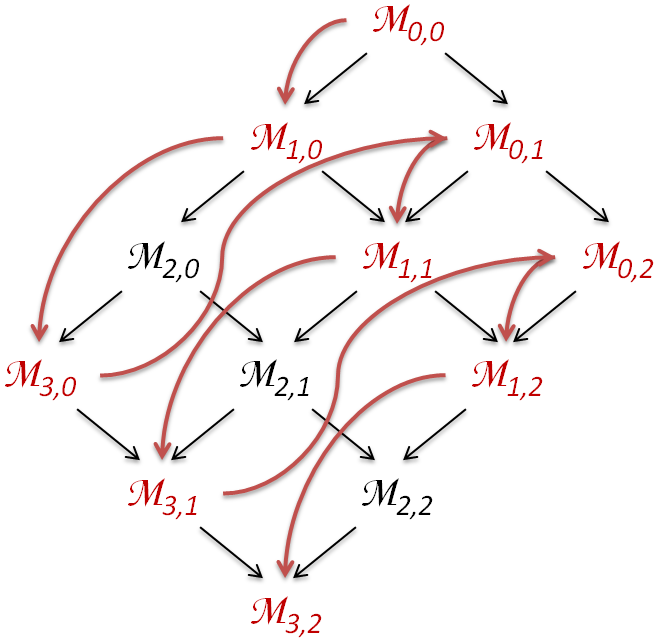
\includegraphics[width=0.75\columnwidth]{img/Pstrat_km_relax.png}
%\caption{The traversal of the lattice by strategy \emph{prune-and-cut}. The highlighted relaxed instances are being solved.}
%\label{fig:example-relax-P}
%\end{figure}


\textbf{Combined Strategy.}
%
The drawback of the \emph{prune-and-cut} strategy is that in the case the makespan needs to be increased, we first increase $k$ up to $k_{max}$ before increasing $m$. To mitigate this problem, we present the \emph{combined} strategy (\ssc{} for short). The initial candidate is again $k=0$ and $m=0$. If the relaxed instance is unsolvable, we increase both $k=k+1$ and $m=m+1$ at the same time. This way, we save solver calls because we do not need to explore all of the possible reductions in the $k$ direction. On the other hand, this strategy is no longer optimal. Figure~\ref{fig:p_counterexample} with blue agent choosing the blue path is a counterexample.
%
\begin{prop}\cite{AAMAS_corridors}
If a MAPF instance $\inst$ has a solution, \emph{combined} strategy is guaranteed to find a solution (completeness) but not necessarily an optimal one.
\end{prop}
%
%\begin{proof}
%If it is necessary to use all of the vertices in the graph $G$ to find a solution, \emph{combined} strategy will eventually increase $k$ up to $k_{max}$ since $k_{max}$ is a finite number. However, in doing so, it may overestimate the $m$ needed. Figure~\ref{fig:p_counterexample} with blue agent choosing the blue path is again such an example.
%\end{proof}
%
\begin{figure}[ht]
\centering
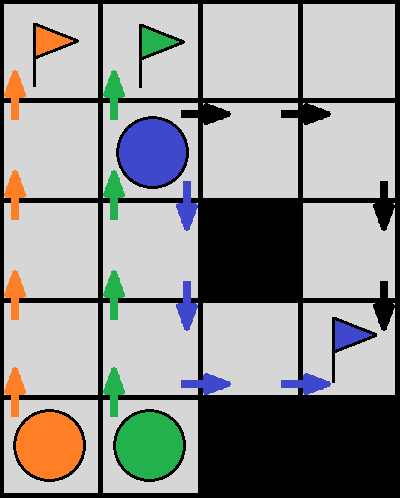
\includegraphics[width=0.3\columnwidth]{img/p_counterexample.png}
\caption{An example instance where the blue agent has two choices of the shortest path. If the blue path is chosen, the proposed strategies perform worse.}
\label{fig:p_counterexample}
\end{figure}
%
%%% Local Variables:
%%% mode: latex
%%% TeX-master: "main"
%%% End:
